% !TeX encoding = UTF-8

% 载入 SJTUThesis 模版
\documentclass[type=bachelor,oneside]{sjtuthesis}
% 选项
%   type=[doctor|master|bachelor],     % 可选(默认:master),论文类型
%   zihao=[-4|5],                      % 可选(默认:-4),正文字号大小
%   lang=[zh|en|de|ja],                % 可选(默认:zh),论文的主要语言
%   review,                            % 可选(默认:关闭),盲审模式
%   [twoside|oneside],                 % 可选(默认:twoside),双页或单页边距模式
%   [openright|openany],               % 可选(默认:openright),奇数页或任意页开始新章
%   math-style=[ISO|TeX],              % 可选 (默认:ISO),数学符号样式
%\usepackage[hidelinks]{hyperref}


% 论文基本配置,加载宏包等全局配置
% !TEX root = ./main.tex

\sjtusetup{
  %
  %******************************
  % 注意:
  %   1. 配置里面不要出现空行
  %   2. 不需要的配置信息可以删除
  %******************************
  %
  % 信息录入
  %
  info = {%
    %
    % 标题
    %
    zh / title           = {上海交通大学本科毕业论文\\2024修订版\LaTeX 模板},
    en / title           = {A \LaTeX \ Template for SJTU\\  Bachelor's Degree Thesis},
    %
    % 标题页标题
    %   可使用“\\”命令手动控制换行
    %
    % 关键词
    %
    zh / keywords        = {落叶的位置,谱出一首诗,时间在消逝,我们的故事开始},
    en / keywords        = {keyword1, keywoerd2,keyword3
    },
    % 姓名
    %
    zh / author          = {你的名字},
    en / author          = {Nide Name},
    %
    % 指导教师
    %
    zh / supervisor      = {某某教授},
    en / supervisor      = {Prof. Uom Uom},
    %
    % 副指导教师
    %
    % assoc-supervisor  = {某某教授},
    % assoc-supervisor* = {Prof. Uom Uom},
    %
    % 学号
    %
    id              = {XXXXXXXXXXXX},
    %
    % 学位
    %   本科生不需要填写
    %
    zh / degree          = {学士},
    en / degree          = {Bachelor of Engineering},
    %
    % 专业
    %
    zh / major           = {请输入你的专业名称},
    en / major           = {Your Major Here},
    %
    % 所属院系
    %
    zh / department      = {请输入你的学院名称},
    en / department      = {Your School Here},
    %
    % 答辩日期
    %   使用 ISO 格式 (yyyy-mm-dd);默认为当前时间
    %
     date                 = {202X-06},
    %
    % 标题页显示日期
    %   覆盖对应标题页的日期显示,原样输出
    %
     zh / display-date    = {202X 年 6 月},
     en / display-date    = {June, 202X},
    %
    % 资助基金
    %
    % zh / fund  = {
    %                {国家 973 项目 (No. 2025CB000000)},
    %                {国家自然科学基金 (No. 81120250000)},
    %              },
    % en / fund  = {
    %                {National Basic Research Program of China (Grant No. 2025CB000000)},
    %                {National Natural Science Foundation of China (Grant No. 81120250000)},
    %              },
  },
  %
  % 风格设置
  %
  style = {%
    %
    % 论文标题页 logo 颜色 (red/blue/black)
    %
    % title-logo-color = black,
  },
  %
  % 名称设置
  %
  name = {
    % bib             = {References},
    % ack             = {谢\hspace{\ccwd}辞},
    % achv            = {攻读学位期间完成的论文},
    digest={},
  },
}

% 使用 BibLaTeX 处理参考文献
%   biblatex-gb7714-2015 常用选项
%     gbnamefmt=lowercase     姓名大小写由输入信息确定
%     gbpub=false             禁用出版信息缺失处理
\usepackage[backend=biber,style=gb7714-2015,gbnamefmt=lowercase]{biblatex}
% 文献表字体
% \renewcommand{\bibfont}{\zihao{5}\fixedlineskip{15.6bp}}
% 文献表条目间的间距
\setlength{\bibitemsep}{0pt}
% 导入参考文献数据库
\addbibresource{refs.bib}

% 脚注格式
\usepackage[perpage,bottom,hang]{footmisc}

% 定义图片文件目录与扩展名
\graphicspath{{figures/}}
\DeclareGraphicsExtensions{.pdf,.eps,.png,.jpg,.jpeg}

% 确定浮动对象的位置,可以使用 [H],强制将浮动对象放到这里(可能效果很差)
\usepackage{float}

% 固定宽度的表格
% \usepackage{tabularx}

% 使用三线表:toprule,midrule,bottomrule。
\usepackage{booktabs}

% 表格中支持跨行
\usepackage{multirow}

% 表格中数字按小数点对齐
\usepackage{dcolumn}
\newcolumntype{d}[1]{D{.}{.}{#1}}

% 使用长表格
\usepackage{longtable}

% 附带脚注的表格
\usepackage{threeparttable}

% 附带脚注的长表格
\usepackage{threeparttablex}

% 算法环境宏包
\usepackage[ruled,vlined,linesnumbered]{algorithm2e}
% \usepackage{algorithm, algorithmicx, algpseudocode}

% 代码环境宏包
\usepackage{listings}
\lstdefinestyle{lstStyleCode}{%
  aboveskip         = \medskipamount,
  belowskip         = \medskipamount,
  basicstyle        = \ttfamily\zihao{6},
  commentstyle      = \slshape\color{black!60},
  stringstyle       = \color{green!40!black!100},
  keywordstyle      = \bfseries\color{blue!50!black},
  extendedchars     = false,
  upquote           = true,
  tabsize           = 2,
  showstringspaces  = false,
  xleftmargin       = 1em,
  xrightmargin      = 1em,
  breaklines        = false,
  framexleftmargin  = 1em,
  framexrightmargin = 1em,
  backgroundcolor   = \color{gray!10},
  columns           = flexible,
  keepspaces        = true,
  texcl             = true,
  mathescape        = true
}
\lstnewenvironment{codeblock}[1][]{%
  \lstset{style=lstStyleCode,#1}}{}

% 直立体数学符号
\providecommand{\dd}{\mathop{}\!\mathrm{d}}
\providecommand{\ee}{\mathrm{e}}
\providecommand{\ii}{\mathrm{i}}
\providecommand{\jj}{\mathrm{j}}

% 化学式
\usepackage[version=4]{mhchem}

% 国际单位制宏包
\usepackage{siunitx}

% 定理环境宏包
\usepackage{ntheorem}
% \usepackage{amsthm}

% 绘图宏包
\usepackage{tikz}
\usetikzlibrary{arrows.meta, shapes.geometric}

% 使用列表
\usepackage{paralist}

% 一些文档中用到的 logo
\usepackage{hologo}
\providecommand{\XeTeX}{\hologo{XeTeX}}
\providecommand{\BibLaTeX}{\textsc{Bib}\LaTeX}

% 借用 ltxdoc 里面的几个命令方便写文档
\DeclareRobustCommand\cs[1]{\texttt{\char`\\#1}}
\providecommand\pkg[1]{{\sffamily#1}}

% hyperref 宏包在最后调用
\usepackage[hidelinks]{hyperref}

% E-mail
\providecommand{\email}[1]{\href{mailto:#1}{\urlstyle{tt}\nolinkurl{#1}}}

%设置标注
\usepackage{caption}
\captionsetup[figure]{belowskip=0pt,aboveskip=1pt}
\captionsetup[table]{belowskip=0.5pt,aboveskip=1pt}

%插入外置原创性声明及使用授权书
\usepackage{pdfpages}

%注释
\usepackage{comment}

%改变字体颜色
\usepackage{color}

\begin{document}
\setlength{\baselineskip}{20pt}

%TC:ignore

% 标题页
\maketitle

% 前置部分
% 请在scan文件夹中替换任务书taskpaper.pdf
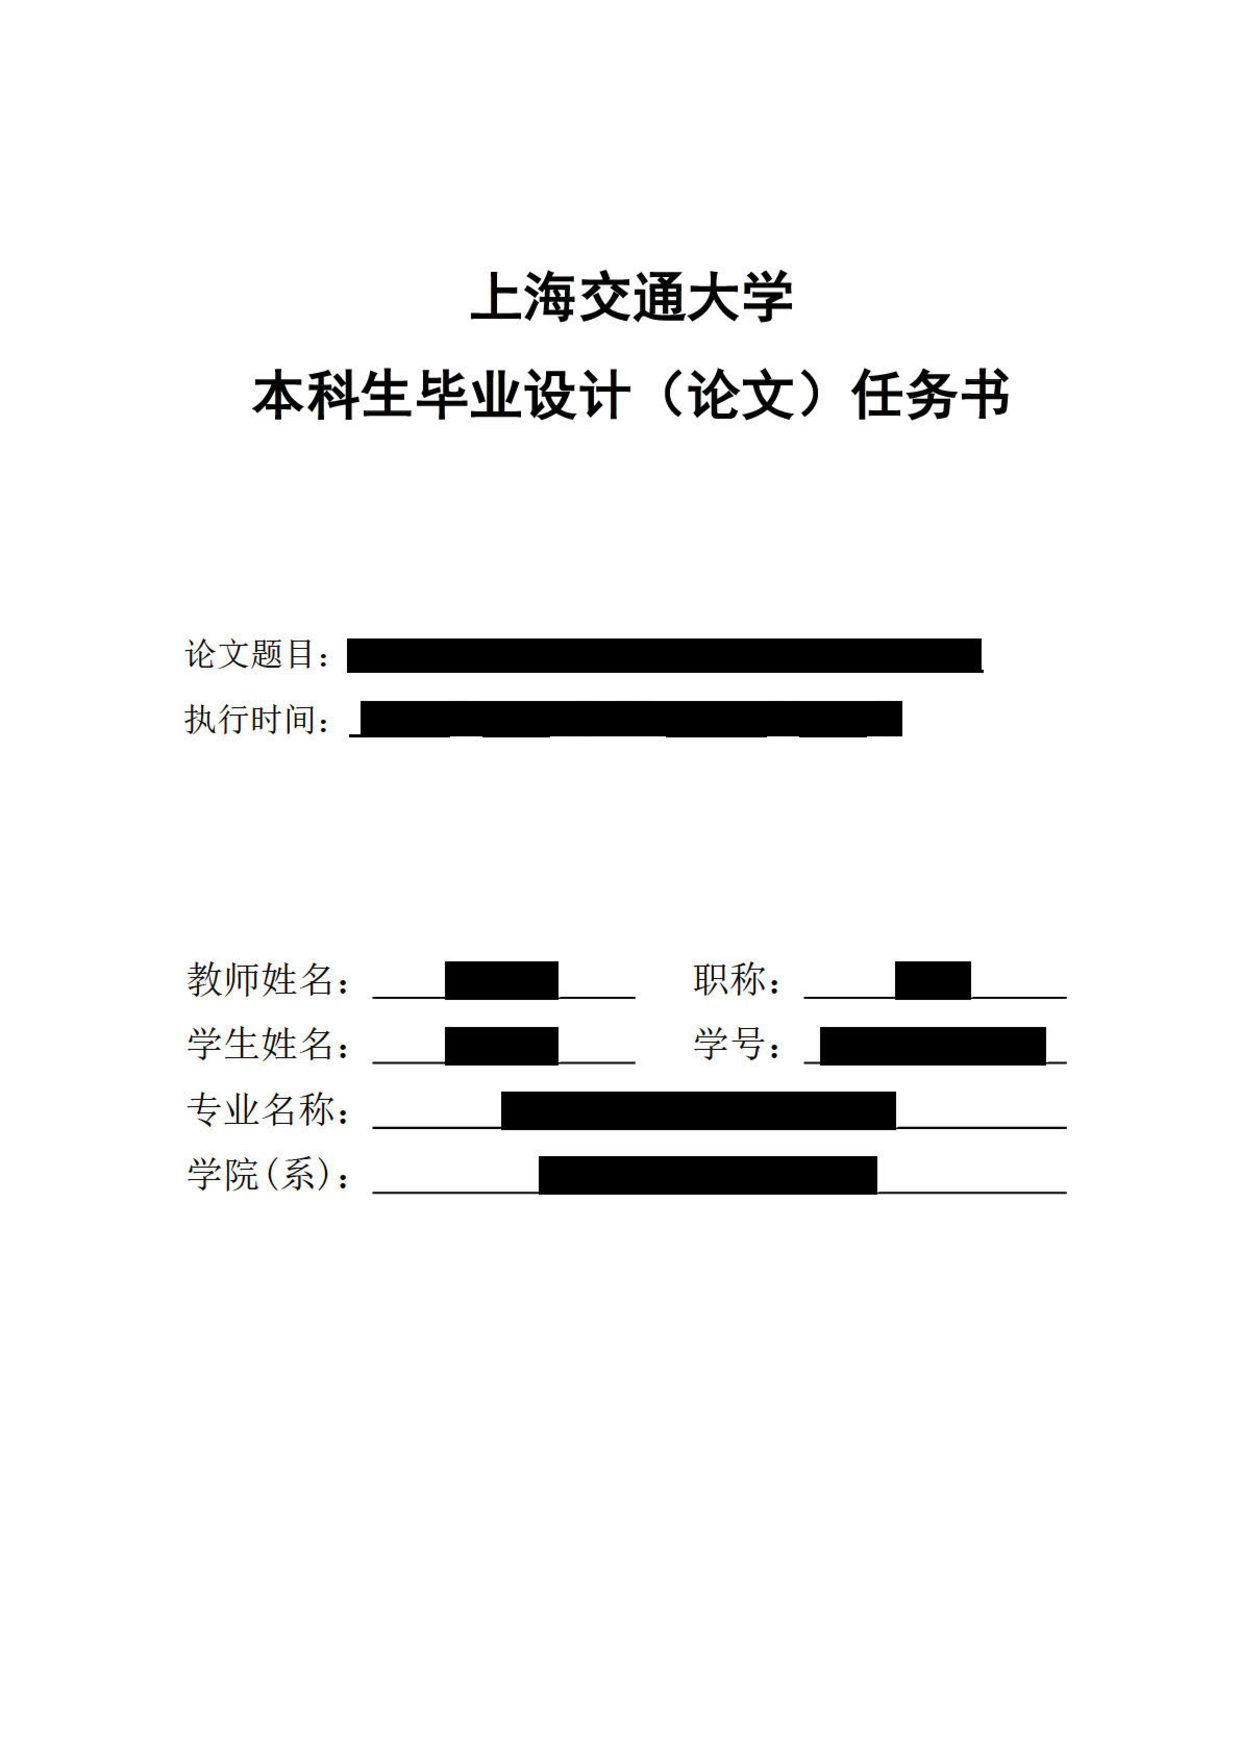
\includepdf[pages={1-4}]{scans/taskpaper.pdf}
% 请在scan文件夹中替换原创性声明及使用授权书copyright.pdf
\copyrightpage[scans/copyright.pdf]

\frontmatter
{
\fancyhead[LE,RO]{}

{
\ctexset{chapter={afterskip=26bp}}
% 摘要
% !TEX root = ../main.tex

\begin{abstract}[zh]
\addcontentsline{toc}{chapter}{摘 \quad 要}
摘要又称内容提要,它应以浓缩的形式概括研究课题的内容、
方法和观点,以及取得的成果和结论,应能反映整个内容的精华。
中英文摘要以 300-500 字为宜(不超过 800 字)。撰写摘要时应
注意以下几点:
\begin{asparaenum}[1)]
\item 用精炼、概括的语言来表达,每项内容不宜展开论证或
说明;
\item 要客观陈述,不宜加主观评价;
\item 成果和结论性字句是摘要的重点,在文字论述上要多些,
以加深读者的印象;
\item 要独立成文,选词用语要避免与全文尤其是前言和结论
部分雷同;
\item 既要写得简短扼要,又要生动,在词语润色、表达方法
和章法结构上要尽可能写得有文彩,以唤起读者对全文阅读的
兴趣。
\end{asparaenum}
\end{abstract}

{
\newfontface{\arial}{Arial}[Scale=0.94]
\ctexset{chapter/format+={\arial}}
\begin{abstract}[en]
\addcontentsline{toc}{chapter}{ABSTRACT}
The abstract, also known as the summary of content, should summarize the content, methods and views of the research topic in a condensed form, as well as the results and conclusions obtained, which should reflect the essence of the entire content. The Chinese and English abstracts should be 300-500 words (not exceeding 800 words). When writing an abstract, the following points should be noted:
\begin{asparaenum}[1)]
	\item Express in concise and generalized language, and each item should not be elaborated or explained;
	\item Objective statements should be made, and subjective evaluations should not be added;
	\item The focus of the abstract should be on the results and conclusive sentences, and there should be more textual discussion to deepen the reader's impression;
	\item To be written independently, the choice of words and language should avoid similarity with the entire text, especially the introduction and conclusion parts;
	\item It should be written in a concise and lively manner, with emphasis on word refinement, expression methods, and organizational structure, in order to arouse readers' interest in reading the entire text.
\end{asparaenum}



\end{abstract}
}
}

{
\ctexset{chapter={afterskip=26bp}}
\renewcommand{\cftchapfont}{\zihao{4}\bfseries}
\renewcommand{\cftsecfont}{\zihao{-4}}
\renewcommand{\cftsubsecfont}{\zihao{5}}
% 目录
\tableofcontents
}
% % 插图索引
% \listoffigures*
% % 表格索引
% \listoftables*
% % 算法索引
% \listofalgorithms*

%TC:endignore
}
% 主体部分
\mainmatter

% 正文内容
{
\ctexset{chapter={afterskip=26bp}}
% !TEX root = ../main.tex

\chapter{绪论}
应说明本课题的意义、目的、研究范围及要求达到的技术参数;简述本课题应解决的主要问题。
\section{研究背景与意义}
\section{研究主要内容}
\section{国内外研究现状}
\section{全文结构}

% !TEX root = ../main.tex

\chapter{正文}

正文是主体,是作者对研究工作的详细表述。理(工)科类正文一般包括本研究内容的总体方案设计与选择论证,各部分(包括硬件与软件)的设计计算,试验方案设计的可行性、有效性以及试验(实验)数据处理及分析,理论分析等。管理人文类学科的论文一般包括对研究问题的论述及系统分析,比较研究,模型或方案设计,案例论证或实证分析,模型运行的结果分析或建议、改进措施等。应对本研究内容及成果进行较全面、客观的理论阐述,应着重指出本研究内容中的创新、改进与实际应用之处。凡引用他人观点、方案、资料、数据等,无论曾否发表,无论是纸质或电子版,均应详加注释。在科学研究和学术活动中的各种造假、抄袭、剽窃和其他违背科学共同体惯例的行为均属学术不端行为。
论文主体各章后应有一节“本章小结”。
\section{二级}
\subsection{三级}
\subsubsection{四级}
\indent
\section{本章小结}
本章干了啥?懒得看那么多正文,看个小结就够了。
\begin{asparaenum}[1)]
	\item 第一点
	\item 第二点
	\item 第三点
\end{asparaenum}



% !TEX root = ../main.tex

\chapter{正文}

正文是主体,是作者对研究工作的详细表述。理(工)科类正文一般包括本研究内容的总体方案设计与选择论证,各部分(包括硬件与软件)的设计计算,试验方案设计的可行性、有效性以及试验(实验)数据处理及分析,理论分析等。管理人文类学科的论文一般包括对研究问题的论述及系统分析,比较研究,模型或方案设计,案例论证或实证分析,模型运行的结果分析或建议、改进措施等。应对本研究内容及成果进行较全面、客观的理论阐述,应着重指出本研究内容中的创新、改进与实际应用之处。凡引用他人观点、方案、资料、数据等,无论曾否发表,无论是纸质或电子版,均应详加注释。在科学研究和学术活动中的各种造假、抄袭、剽窃和其他违背科学共同体惯例的行为均属学术不端行为。
论文主体各章后应有一节“本章小结”。
\section{二级}
\subsection{三级}
\subsubsection{四级}
\indent
\section{本章小结}
本章干了啥?懒得看那么多正文,看个小结就够了。
\begin{asparaenum}[1)]
	\item 第一点
	\item 第二点
	\item 第三点
\end{asparaenum}



% !TEX root = ../main.tex

\chapter{正文}

正文是主体,是作者对研究工作的详细表述。理(工)科类正文一般包括本研究内容的总体方案设计与选择论证,各部分(包括硬件与软件)的设计计算,试验方案设计的可行性、有效性以及试验(实验)数据处理及分析,理论分析等。管理人文类学科的论文一般包括对研究问题的论述及系统分析,比较研究,模型或方案设计,案例论证或实证分析,模型运行的结果分析或建议、改进措施等。应对本研究内容及成果进行较全面、客观的理论阐述,应着重指出本研究内容中的创新、改进与实际应用之处。凡引用他人观点、方案、资料、数据等,无论曾否发表,无论是纸质或电子版,均应详加注释。在科学研究和学术活动中的各种造假、抄袭、剽窃和其他违背科学共同体惯例的行为均属学术不端行为。
论文主体各章后应有一节“本章小结”。
\section{二级}
\subsection{三级}
\subsubsection{四级}
\indent
\section{本章小结}
本章干了啥?懒得看那么多正文,看个小结就够了。
\begin{asparaenum}[1)]
	\item 第一点
	\item 第二点
	\item 第三点
\end{asparaenum}



% !TEX root = ../main.tex

\chapter{正文}

正文是主体,是作者对研究工作的详细表述。理(工)科类正文一般包括本研究内容的总体方案设计与选择论证,各部分(包括硬件与软件)的设计计算,试验方案设计的可行性、有效性以及试验(实验)数据处理及分析,理论分析等。管理人文类学科的论文一般包括对研究问题的论述及系统分析,比较研究,模型或方案设计,案例论证或实证分析,模型运行的结果分析或建议、改进措施等。应对本研究内容及成果进行较全面、客观的理论阐述,应着重指出本研究内容中的创新、改进与实际应用之处。凡引用他人观点、方案、资料、数据等,无论曾否发表,无论是纸质或电子版,均应详加注释。在科学研究和学术活动中的各种造假、抄袭、剽窃和其他违背科学共同体惯例的行为均属学术不端行为。
论文主体各章后应有一节“本章小结”。
\section{二级}
\subsection{三级}
\subsubsection{四级}
\indent
\section{本章小结}
本章干了啥?懒得看那么多正文,看个小结就够了。
\begin{asparaenum}[1)]
	\item 第一点
	\item 第二点
	\item 第三点
\end{asparaenum}



% !TEX root = ../main.tex

\chapter{全文总结}

\section{主要结论}
全文总结(结语)包括对整个研究工作进行归纳和综合而得出的总结,还应包括所得结果与已有结果的比较和本课题尚存在的问题,以及进一步开展研究的见解与建议。结论集中反映作者的研究成果,表达作者对所研究的课题的见解,是全文的思想精髓,是文章价值的体现,结论要写得概括、简短。撰写时应注意以下几点。
\begin{asparaenum}[1)]
	\item 全文总结(结语)要简洁、明确,措辞应严密,且又容易被人领会;
	\item 全文总结(结语)应反映自己的研究工作;
	\item  要实事求是地介绍自己的研究成果,切忌言过其实,在无充分把握时应留有余地,因为科学问题的探索是永无止境的。
\end{asparaenum}

}

%TC:ignore

\clearpage
{
\ExplSyntaxOn
\bool_if:NTF \g__sjtu_twoside_bool
{
    \fancyhead [ LE ]     { 参考文献 }
    \fancyhead [ RO ]     { 参考文献 }
}
{
    \fancyhead [ R ] { 参考文献 }
}
\ExplSyntaxOff
% 文献表字体
\renewcommand{\bibfont}{\zihao{5}}
% 设定固定间距
\fixedlineskip{15.6bp}
{
\ctexset{chapter={afterskip=26bp}}
% 参考文献
\printbibliography[heading=bibintoc]
}
\clearpage
}

\makeatletter
% \appendix采用数字编号。
\renewcommand{\appendix}{\par
    \setcounter{chapter}{0}
    \setcounter{section}{0}
    \ctexset{chapter/number={\arabic{chapter}}}
}
% 使用 \appchapter 替代附录中的 \chapter 章节,附录中的章节不再放入目录。
\newcommand{\appchapter}[1]{
    \refstepcounter{chapter}
    \SJTU@head*[附录 \thechapter]{#1(附录 \thechapter)}
}
\makeatother

{
\ctexset{chapter={afterskip=26bp}}
% 附录
\appendix
% 附录中图表不加入索引
\captionsetup{list=no}
\addcontentsline{toc}{chapter}{附\quad 录}
% 插入附录
\appchapter{对\LaTeX 不熟悉可以参考这里}\label{chap:sample}
\textbf{\color{blue}编号条目使用asparaenum编写较为紧凑美观:}
\begin{asparaenum}[1)]
	\item 固体氧化物燃料电池功重比低。
	\item 无涡轮燃烧室流场组织复杂、易出现燃烧不均匀。
\end{asparaenum}

\textbf{\color{blue}公式编写示例如下。}SOFC电池反应\cite{Fu2021}:
\begin{center}
	阳极:\ce{H_2 + O^2- -> H_2O + 2e^-};阴极:\ce{1/2O_2 + 2e^- -> O^2-}
\end{center}

电池中的电化学反应产生电能,电池电流即为电子传输速率,电流大小反映了电化学反应的剧烈程度,如式\eqref{icell}所示:
\begin{equation}
	i=\frac{dQ}{dt}=nF\frac{dN}{dt}=jA
	\label{icell}
\end{equation}

其中,$Q$为总电荷量,$n$为电子迁移量,$N$为物质的量,$j$为电流密度,$A$为反应面积。

多孔介质中气体流动并不缓慢因此不能直接使用Darcy扩散方程而要使用Brinkman方程\eqref{momentumGDE}\cite{Chellehbari2021,Celik2018}。
\begin{align}
	\nabla\left(\rho\textbf{u}\right)&=0\label{mass}\\
	\rho(\textbf{u}\nabla)\textbf{u}&=
	-\nabla p
	+\nabla\left[\mu\left(\nabla \textbf{u}+(\nabla \textbf{u})^{T}\right)-\frac{2\mu}{3}\left(\nabla{\textbf{u}}\right)\right]
	+\textbf{F}\label{momentum}\\
	\nabla(\rho{\textbf{u}})&=Q_{br}\label{massGDE}\\
	\frac{\rho}{\varepsilon^2}\left(\left(\textbf{u} \nabla\right)\textbf{u}\right)&={F}-\nabla{p}+
	\nabla\left[\frac{\mu}{\varepsilon}\left(\nabla{\textbf{u}}
	+\left(\nabla{\textbf{u}}\right)^{T}\right)
	-\frac{2\mu}{3\varepsilon}\left(\nabla{\textbf{u}}\right)\right]
	-\left(\frac{\mu}{\kappa}+
	\frac{Q_{br}}{\varepsilon^{2}}\right)\textbf{u}\label{momentumGDE}
\end{align}

\textbf{\color{blue} 各种图片的插入和引用格式,如图\ref{energypd}、图\ref{Yang2022}、图\ref{resultCCcloud}所示。目前使用[H]需要自行调节每个图片/表格的位置和大小以达到最佳的排版效果(也可以结合vspace\{\}或hspace\{\}指令调整间距),否则如果某页图片放不下则会跳转到下一页,原先位置出现大段留白。但是用htbp会导致图片固定在下一页页首(或b、p位置),后续段落被打断,部分文字前提填补上一页空白,剩下的部分在图片后。最好的方式是如果图片放不下就放在下一段结尾处(而不是页首)。目前还没有研究出自动化解决方案,如果有麻烦告诉我,wx:hello\_rua}
\begin{figure}[H]
	\centering
	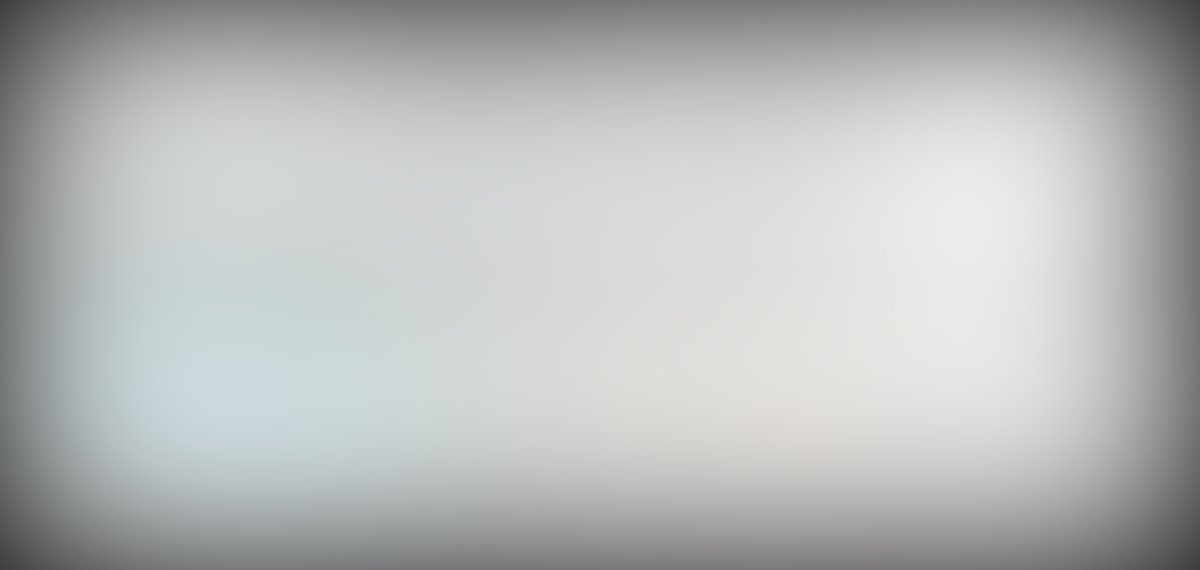
\includegraphics[width=0.9\textwidth]{energypd.jpg}
	\caption{国际能源署2050净零方案关键里程碑图\cite{Chappell2021}}\label{energypd}
\end{figure}
\begin{figure}[H]
	\centering
	\subcaptionbox{同向流和逆向流}[14cm]{
		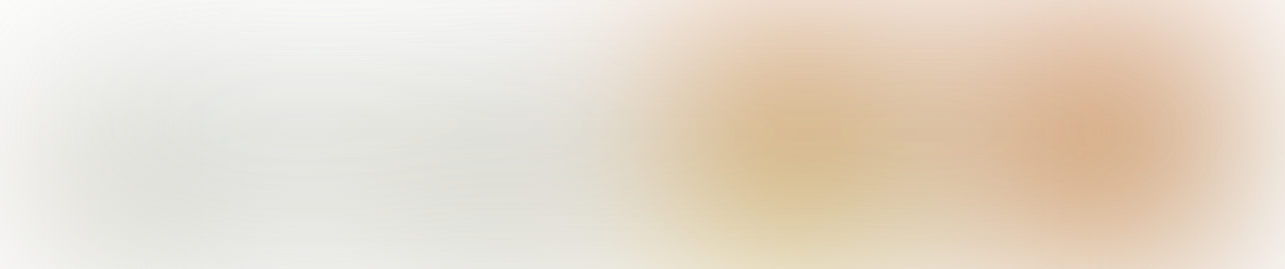
\includegraphics[width=0.75\textwidth]{direction1.png}
	}
	\subcaptionbox{交叉流}[14cm]{
		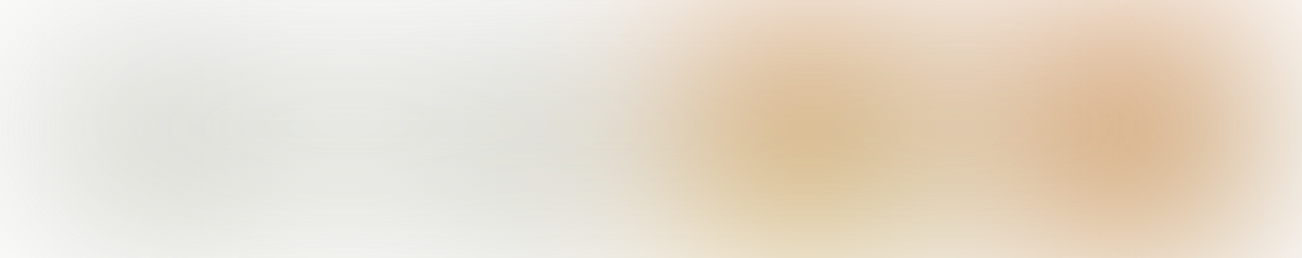
\includegraphics[width=0.75\textwidth]{direction2.png}
	}
	\caption{不同的流动方向及其电流密度分布图\cite{Yang2022}}\label{Yang2022}
\end{figure}
\begin{figure}[H]
	\centering
	\subcaptionbox{COMSOL出口速度云图}[6cm]{
		
\includegraphics[height=3.5cm]{outCOMSOL.png}
	}
	\subcaptionbox{COMSOL横向速度云图}[6cm]{
		
\includegraphics[height=3.5cm]{hCOMSOL.png}
	}
	\subcaptionbox{CFX出口速度云图}[6cm]{
		
\includegraphics[height=3.5cm]{outCFX.png}
	}
	\subcaptionbox{CFX横向速度云图}[6cm]{
		
\includegraphics[height=3.5cm]{hCFX.png}
	}
	\caption{计算结果对比图}\label{resultCCcloud}
\end{figure}
\textbf{\color{blue}表格格式如表\ref{Sasi2024}所示。}
\begin{table}[H]
	\centering
	\caption{氨氢物化性质表\cite{Sasi2024}}\label{Sasi2024}
	\begin{tabular}{ccc}
		\toprule%第一道横线
		&氨&氢\\
		\midrule%第二道横线
		密度(kg/m$^3$)&684&71.4\\
		沸点(K)&239.1&21\\
		分子质量(g/mol)&17&2\\
		低位热值(MJ/kg)&18.61&120\\
		比热容(kJ/kg$\cdot$K)&4.6&8.68\\
		燃点(K)&630&560\\
		\bottomrule%第三道横线
	\end{tabular}
\end{table}
% !TEX root = ../main.tex

\appchapter{符号与标记}\label{chap:symbol}
\begin{tabular}{l}
	$\textbf{u}$——速度矢量\\
	$\rho$——密度\\
	$p$——压强\\
	$\varepsilon$——孔隙率\\
	$\tau$——多孔介质孔道迂曲度\\
	$\kappa$——多孔介质渗透率张量\\
	$\textbf{F}$——体积力矢量\\
	$T$——绝对温度\\
	$\nu_i$——组分i的化学计量系数\\
	$M_i$——组分i的摩尔质量\\
	$F$——法拉第常数\\
	$\omega_i$——组分i的质量分数\\
	$x_i$——组分i的摩尔分数\\
	$R_i$——组分i的电化学反应质量通量\\
	$p_{atm}$——环境大气压\\
	$D_i^{\mathrm{eff}}$——组分i的有效扩散系数\\
	$\lambda_{path}$——分子平均自由程\\
	$M_i$——组分i的摩尔质量\\
	$k_d$——参考扩散系数\\
	$v_i$——组分i的动力学体积\\
	$Q_h$——电化学反应热源\\
	$C_p$——比热容\\
	$k^{\mathrm{eff}}$——有效导热系数\\
	$\Delta s_e$——电化学反应熵变\\
\end{tabular}


% !TEX root = ../main.tex

\appchapter{部份零件工程图}\label{chap:manufac}

\begin{figure}[htbp!]
	\centering
	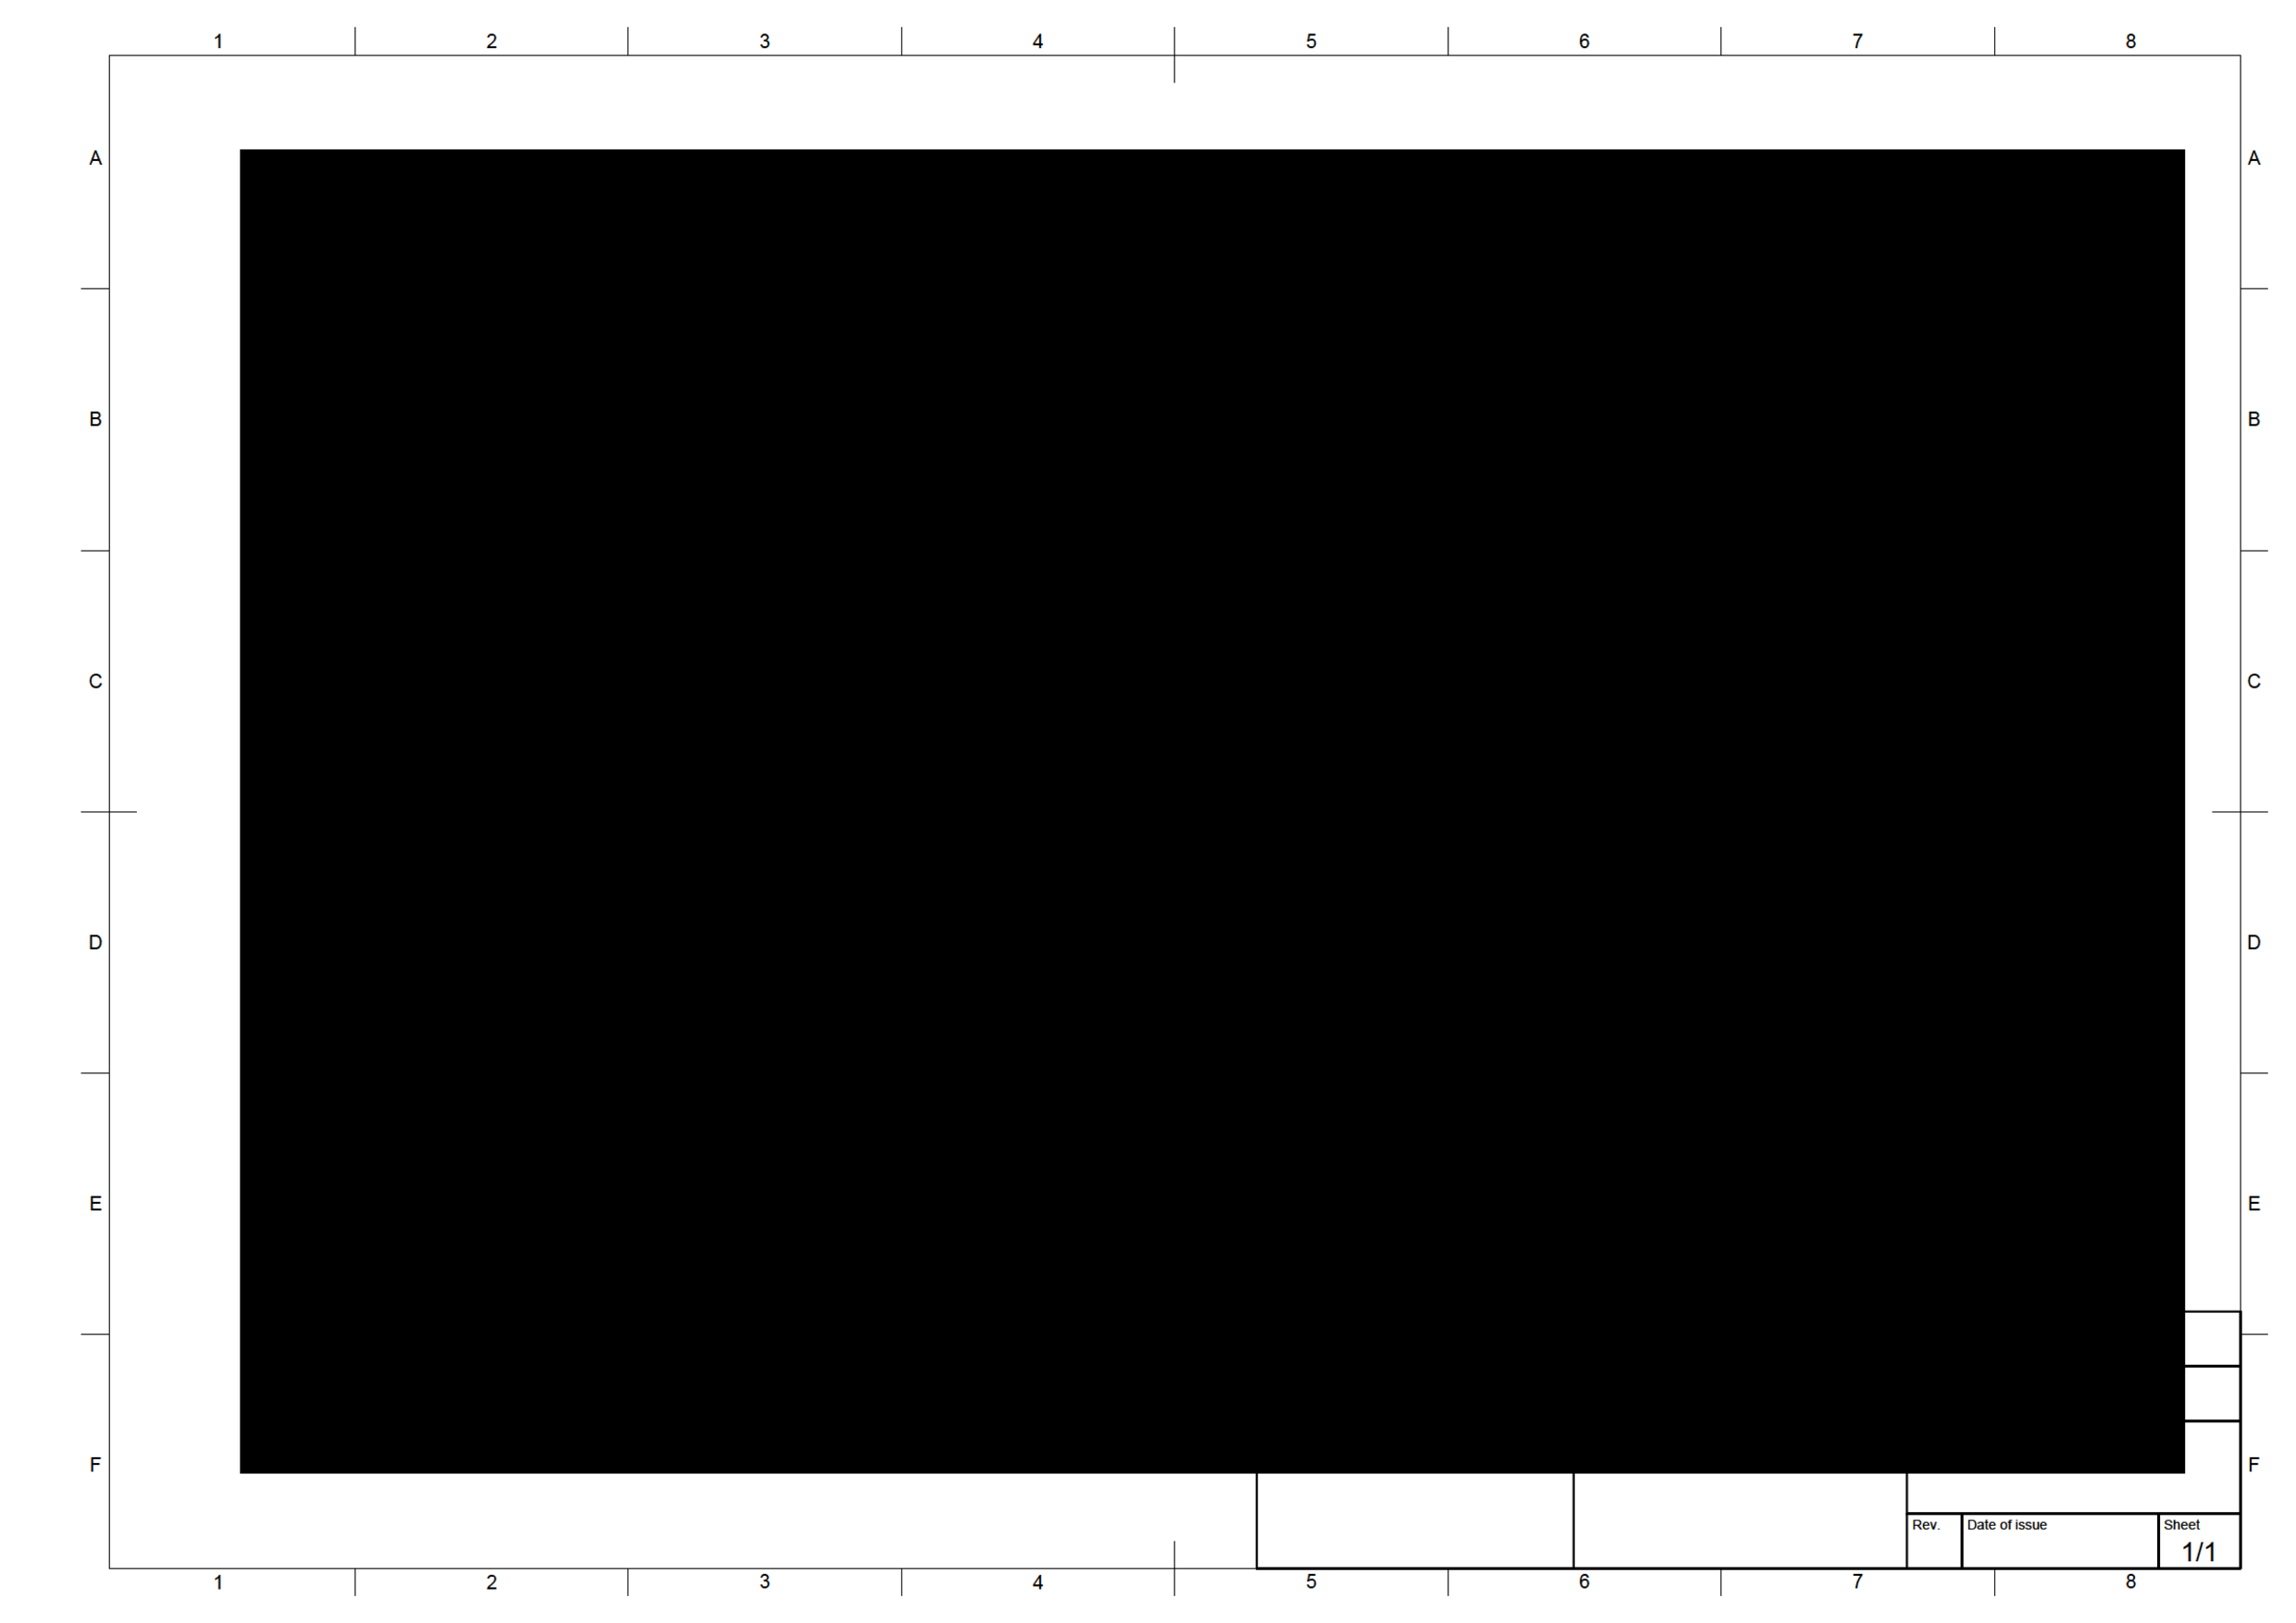
\includegraphics[width=0.875\textwidth]{火焰筒前端板.pdf}
	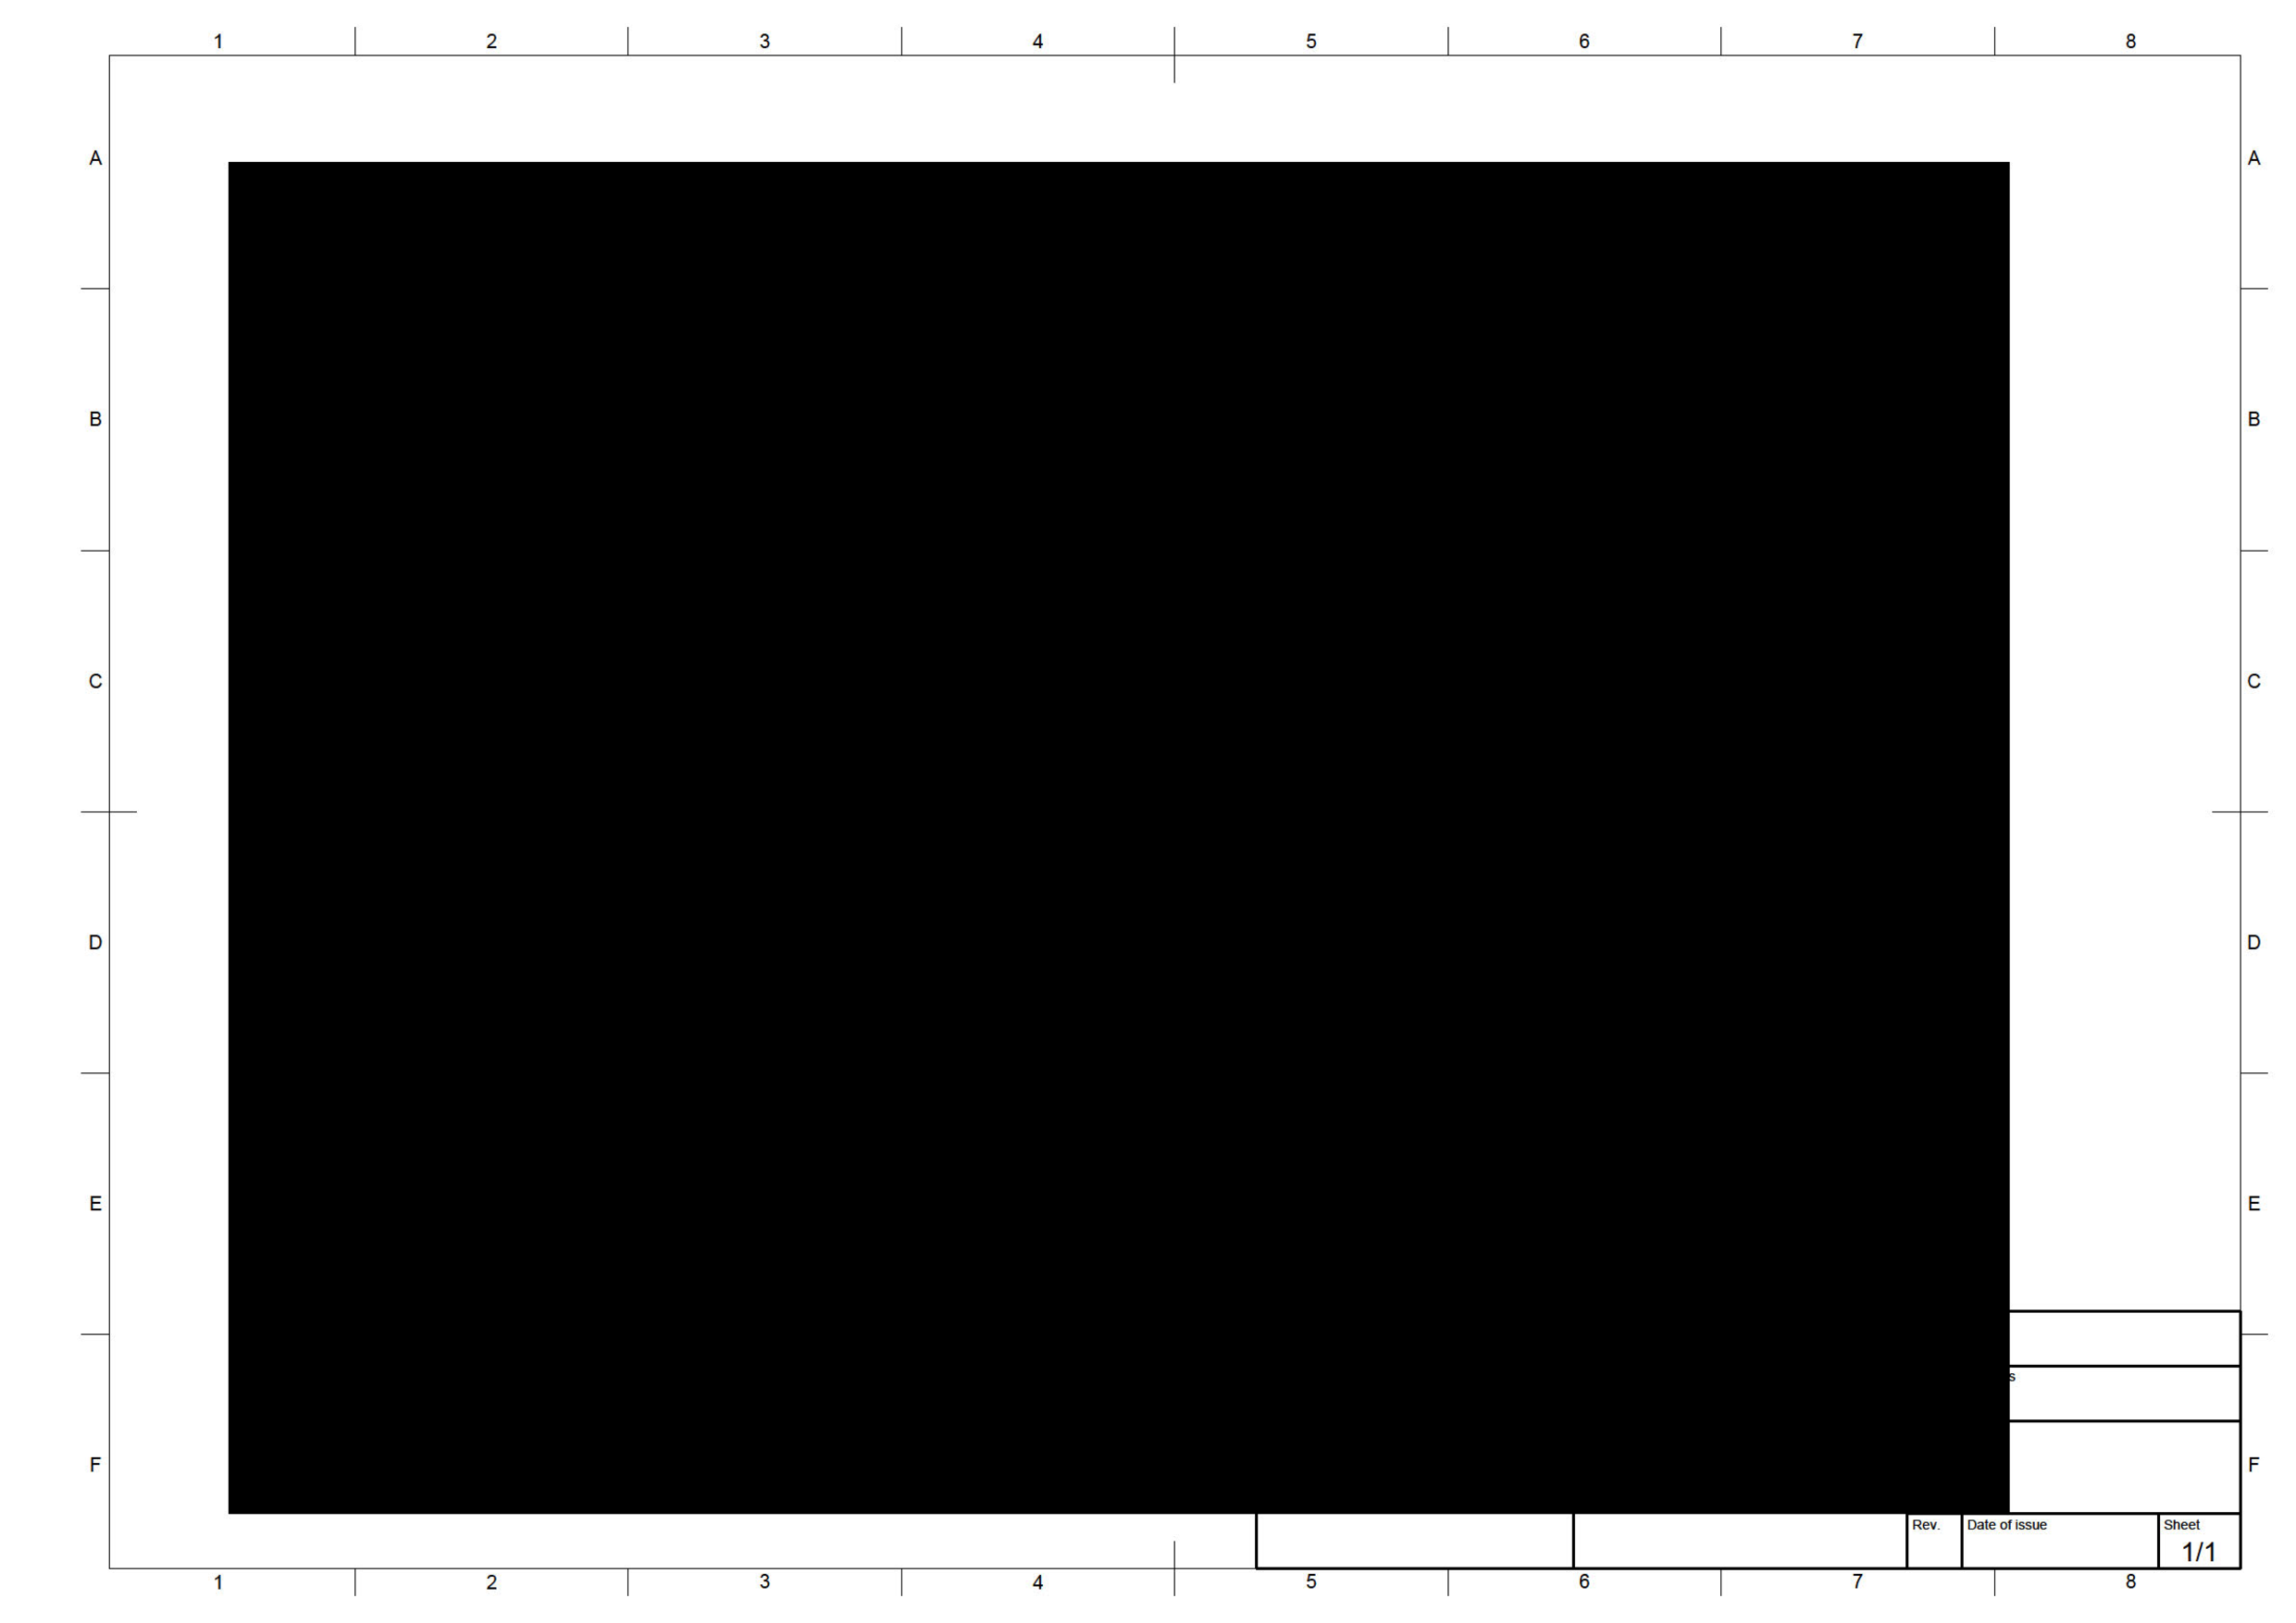
\includegraphics[width=0.875\textwidth]{旋流器.pdf}
	%\caption{}\label{}
\end{figure}
\begin{figure}[htbp!]
	\centering
	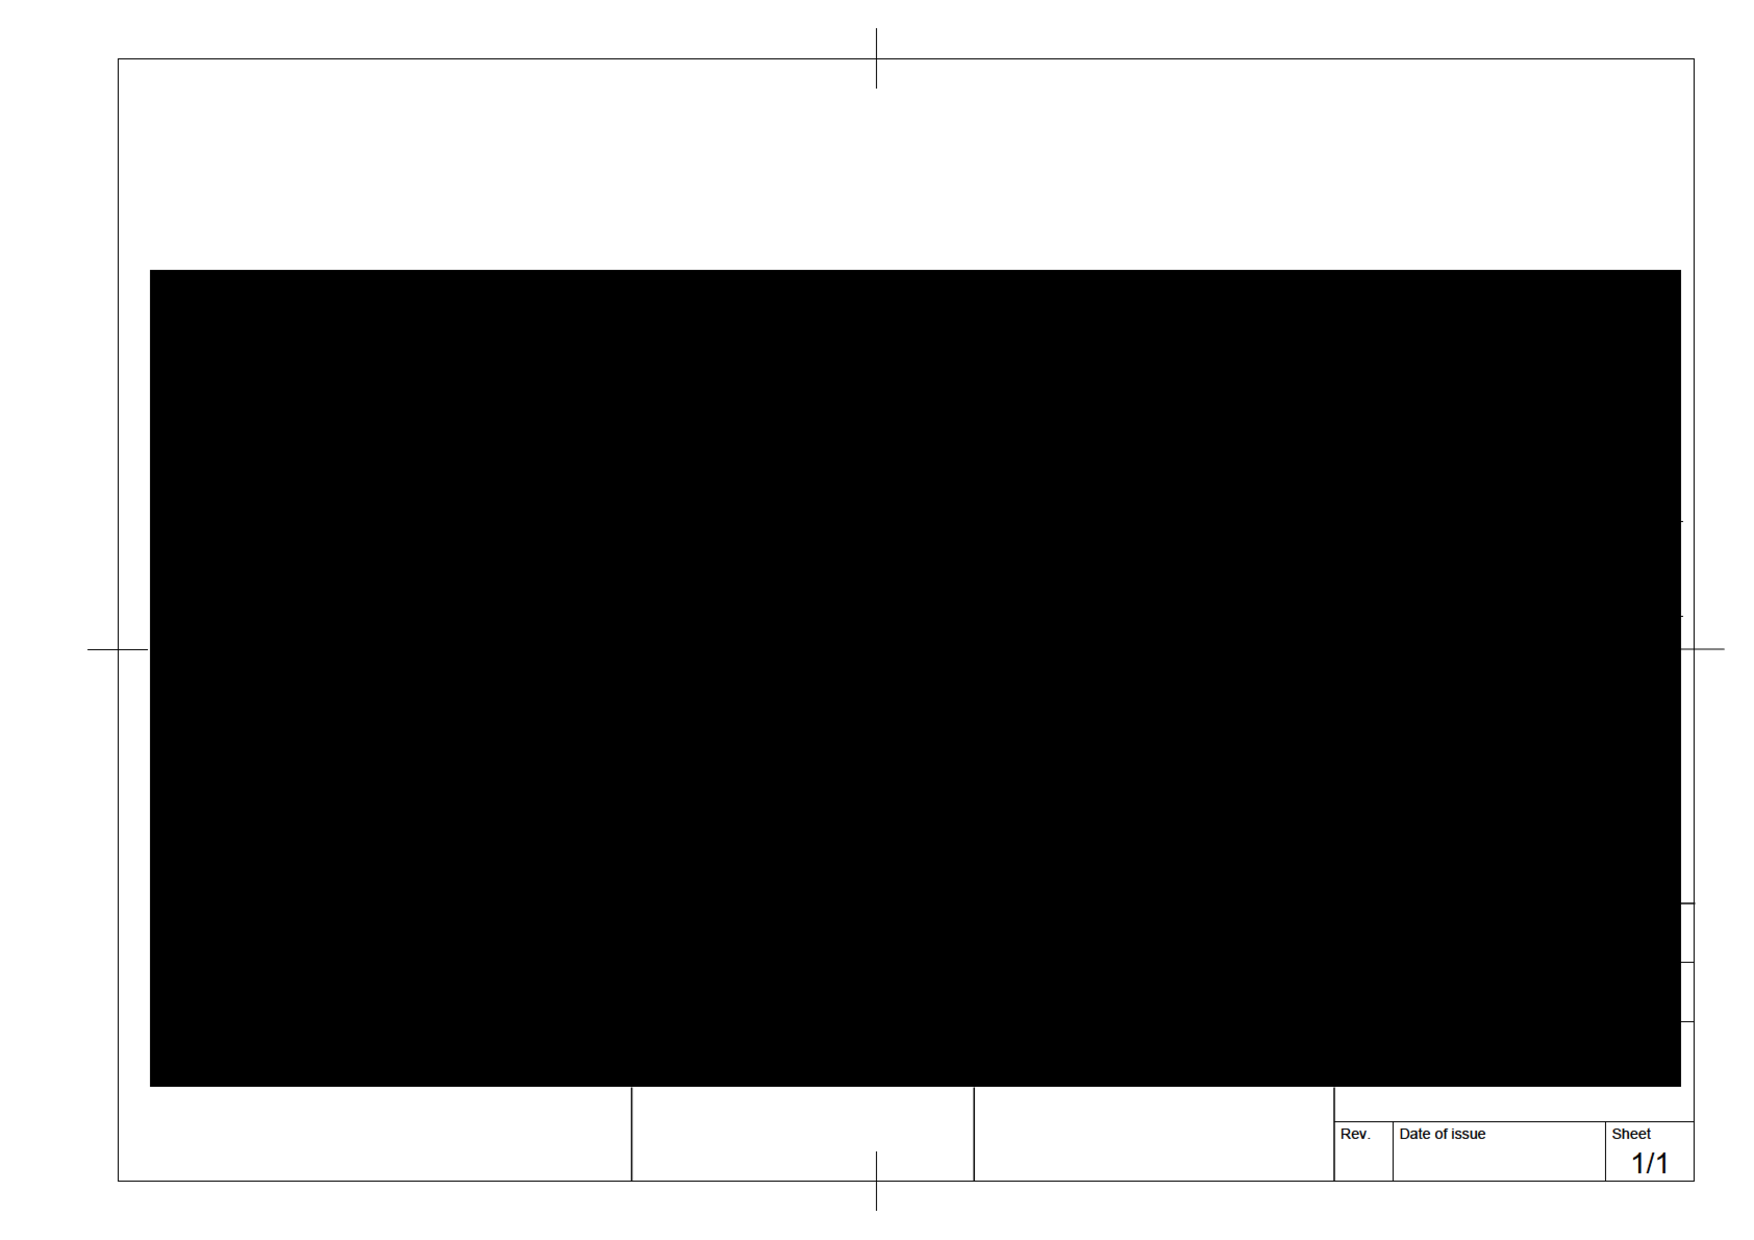
\includegraphics[width=0.875\textwidth]{测温管.pdf}
	%\caption{}\label{}
\end{figure}

\begin{figure}[htbp!]
	\centering
	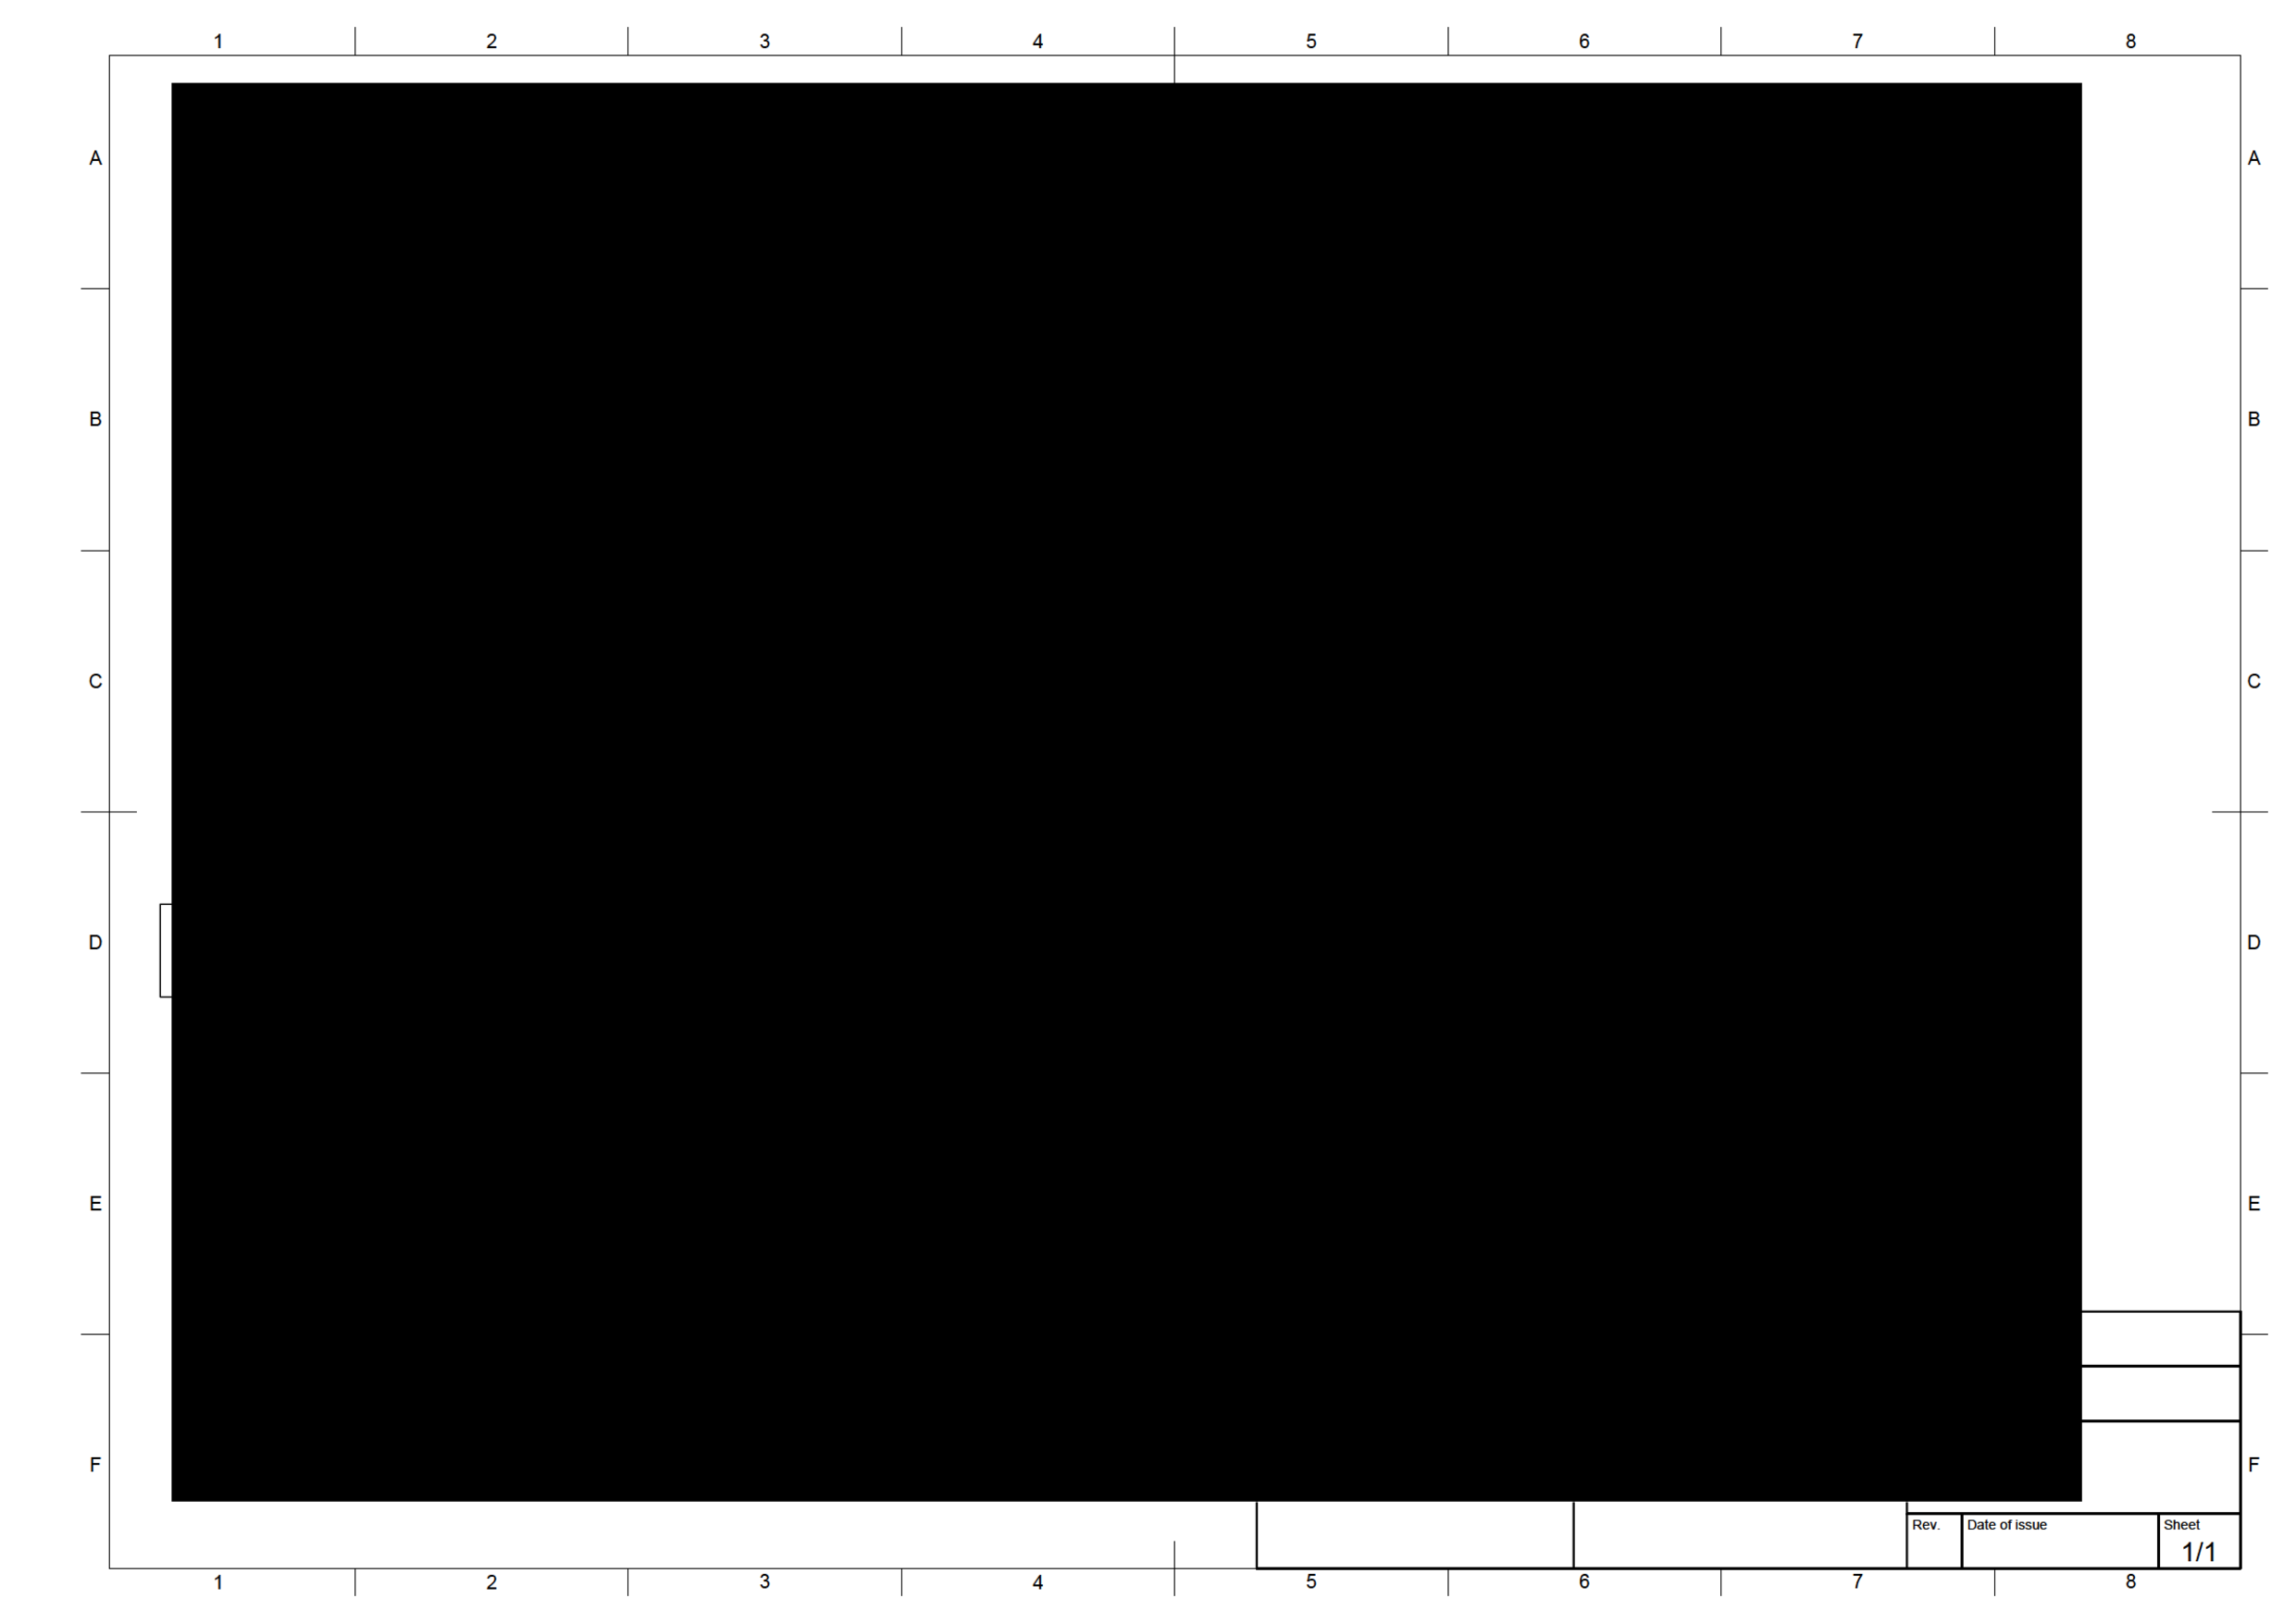
\includegraphics[width=0.875\textwidth]{下支撑架.pdf}
	%\caption{}\label{}
\end{figure}
}


% 结尾部分
\backmatter

{
\ctexset{chapter={afterskip=26bp}}
% 发表论文及科研成果
% !TEX root = ../main.tex

\begin{achievements}

\begin{bibliolist}{00}
  \item 如果没有可以删除本页

\end{bibliolist}


\end{achievements}

}

\clearpage
{
\ExplSyntaxOn
\bool_if:NTF \g__sjtu_twoside_bool
{
    \fancyhead [ LE ]     { 致谢 }
    \fancyhead [ RO ]     { 致谢 }
}
{
    \fancyhead [ R ] { 致谢 }
}
\ExplSyntaxOff
{
\ctexset{chapter={afterskip=26bp}}
% 致谢
% !TEX root = ../main.tex

\begin{acknowledgements}
致谢应以简短的文字对课题研究与论文撰写过程中曾直接给予帮助的人员(例如指导教师、答疑教师及其他人员)表示自己的谢意,这不仅是一种礼貌,也是对他人劳动的尊重,是治学者应当遵循的学术规范。
%署名居中居右
\begin{table}[H]
	\flushright
	\normalsize
	\begin{tabular}{c}
		你的名字\\
		某年某月某日\quad 于某地\\
	\end{tabular}
\end{table}
\end{acknowledgements}

}

\clearpage
}

{
\ctexset{chapter={afterskip=26bp}}
% 学士学位论文要求在最后有一个大摘要,单独编页码
% !TEX root = ../main.tex

\begin{digest}
大摘要是对研究课题的内容、方法和观点,以及取得的成果和结论的凝练。其内容一般应说明本项研究工作的目的和意义、研究方法、实验方法、研究成果、结果和最终结论等,重点是结果和结论,应注意突出论文中具有创新性的成果和独到见解的部分。
\end{digest}

}

\end{document}
